% The Clever Algorithms Project: http://www.CleverAlgorithms.com
% (c) Copyright 2011 Jason Brownlee. Some Rights Reserved. 
% This work is licensed under a Creative Commons Attribution-Noncommercial-Share Alike 2.5 Australia License.

% Name
% The algorithm name defines the canonical name used to refer to the technique, in addition to common aliases, abbreviations, and acronyms. The name is used in terms of the heading and sub-headings of an algorithm description.
\section{Multivariate Adaptive Regression Splines} 
\label{sec:mars}
\index{Multivariate Adaptive Regression Splines}
\index{MARS}
\index{MARSplines}
\index{Adaptive Regression Splines}

% other names
% What is the canonical name and common aliases for a technique?
% What are the common abbreviations and acronyms for a technique?
\emph{Multivariate Adaptive Regression Splines, MARS, MARSplines, Adaptive Regression Splines.}

% Taxonomy: Lineage and locality
% The algorithm taxonomy defines where a techniques fits into the field, both the specific subfields of Computational Intelligence and Biologically Inspired Computation as well as the broader field of Artificial Intelligence. The taxonomy also provides a context for determining the relation- ships between algorithms. The taxonomy may be described in terms of a series of relationship statements or pictorially as a venn diagram or a graph with hierarchical structure.
\subsection{Taxonomy}
% To what fields of study does a technique belong?
Multivariate Adaptive Regression Splines is a Multivariate Non-Parametric Regression method.
% What are the closely related approaches to a technique?
It is related to other Non-Parametric Regression methods such as Kernel Regression, Non-Parametric Multiplicative Regression, Additive Modeling and Regression Trees. The procedure to prepare the model is related to Regressive Partitioning for decision trees (CART). The use of forward and backward phases in regression shows some similarity to Stepwise Regression.
% extensions
Fast MARS in an extension of the canonical MARS method that suggests an optimization of the forward procedure when building the model.
% PolyMars?

% Strategy: Problem solving plan
% The strategy is an abstract description of the computational model. The strategy describes the information processing actions a technique shall take in order to achieve an objective. The strategy provides a logical separation between a computational realization (procedure) and a analogous system (metaphor). A given problem solving strategy may be realized as one of a number specific algorithms or problem solving systems. The strategy description is textual using information processing and algorithmic terminology.
\subsection{Strategy}
% What is the information processing objective of a technique?
The information processing objective of the technique is to find an equation that best describes the relationships between independent and a dependent variable.
% What is the model?
This is achieved by preparing a model that is the weighted sum of basis functions. A basis function can be as simple as a constant, or as complex as one or the product of multiple sub-functions that add non-linearities called hinge functions. Hinge functions take the form of $max(0, x-c)$ where $0$ is the minimum value for the function, $x$ is the variable, and $c$ is a constant (that provides a kink or sharp turn in one-dimension) called the knot. The number of basis functions as well as the parameters for each are determined automatically through an iterative process based on the data.

% what is the algorithm to arrive at the model?
MARS is motivated as a process to create a continuous model using a procedure like that used in recursive partitioning (CART). Like recursive partitioning, the method has a forward procedure to add terms and a backward procedure to prune terms from the model.
% forward
The forward procedure is a greedy algorithm that seeks to minimizes the Sum of Squared Residual (SSR) errors. It starts with the intercept and adds basis function terms to the model until a maximum number of terms have been added or no further improvements in SSR are possible. Terms are added and configured to give the greatest reduction in SSR.

% backward
The intent of the forward procedure is overfit the training data. The backward step is intended to add generality to the mode by pruning terms one-at-a-time selecting each term to remove based on the improvement in a generalized cross-validation score. The backward pass typically prunes one side of each pair of terms.
% cross validation score
The generalized cross-validation score is a performance measure that takes the complexity of the model and size of the training dataset as well as the SSR into account. The score seeks to minimize for model flexibility.

% Heuristics: Usage guidelines
% The heuristics element describe the commonsense, best practice, and demonstrated rules for applying and configuring a parameterized algorithm. The heuristics relate to the technical details of the techniques procedure and data structures for general classes of application (neither specific implementations not specific problem instances). The heuristics are described textually, such as a series of guidelines in a bullet-point structure.
\subsection{Heuristics}
% What are the suggested configurations for a technique?
% What are the guidelines for the application of a technique to a problem instance?

\begin{itemize}
	\item Friedman originally proposed it a suitable technique for sample sizes $50 \leq N \leq 1000$ and dimensions $3 \leq n \leq 20$.
	\item The algorithm requires the specification of the maximum number of terms to add in the forward pass. % recommended values?
	\item A penalty term (\texttt{d}) is used on the generalized cross-validation score which is commonly set to a small integer value ($d<4$, typically 2 or 3).
	\item Constraints can be imposed on the addition of terms in the forward pass, such as limitations on the number of interactions permitted between basis functions. Low numbers of interactions are common (such as 1 or 2).
	\item It may be more suitable to real valued variables than recursive partitioning given the continuous nature of the hinge basis functions.
	\item Like partitioning, data preparation may not required as the hinge functions can account for outliers.
	\item The training times for MARS are relatively fast although it is a generally slower process to fit than Recursive Partitioning on the same training dataset.
\end{itemize}

% sample script in R
\subsection{Code Listing}
% listing
Listing~\ref{earth_multivariate_adaptive_regression_splines} provides a code listing Multivariate Adaptive Regression Splines method in R to find a line of best fit for a two-dimensional data set.
Figure~\ref{plot:multivariate_adaptive_regression_splines_result} provides a plot of the training dataset with the line of best fit highlighted.

% algorithm and package
The example uses the \texttt{earth()} function in the \texttt{earth} package that uses a generalized linear model as the underling method and provides access to Fast MARS features \cite{Milborrow2012}. For more information on this library type: \texttt{library(help="earth")}, and for more information on the function type: \texttt{?earth}.

% problem
The test problem is a two-dimensional dataset of 50 samples, where the \texttt{x}-values are drawn from a uniformly random distribution $x \in [0,10]$ and \texttt{y} values are the \texttt{x} value plus a value drawn from a normally random distribution with a mean of $0$ and a standard deviation of $1$.

% code listing
\lstinputlisting[firstline=7,language=r,caption={Example of Multivariate Adaptive Regression Splines in R using the \texttt{earth} function of the \texttt{earth} package.}, label=earth_multivariate_adaptive_regression_splines]{../src/algorithms/regression/earth_multivariate_adaptive_regression_splines.R}

\begin{figure}[htp]
\centering
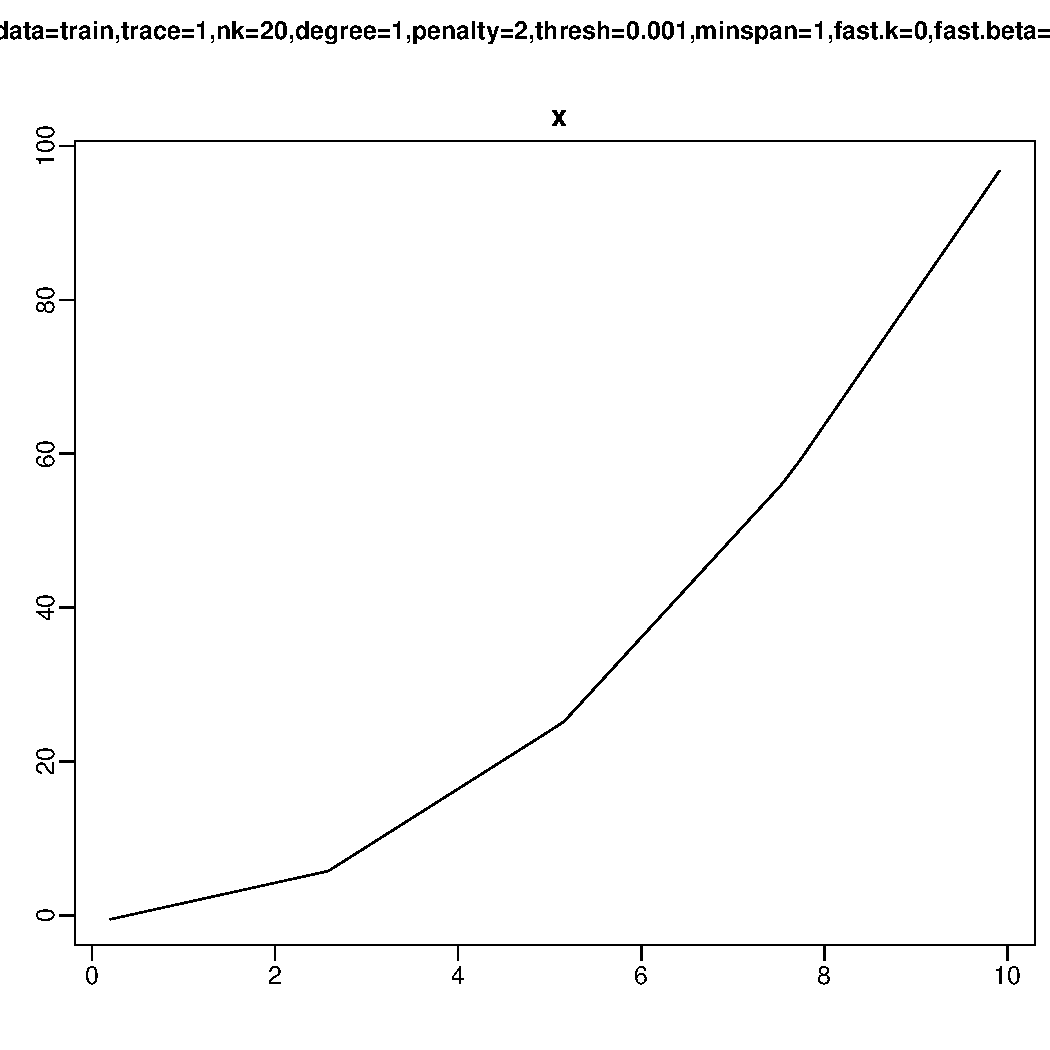
\includegraphics[scale=0.45]{a_regression/multivariate_adaptive_regression_splines_result.pdf}
\caption{Plot 2D showing the line of best fit.}
\label{plot:multivariate_adaptive_regression_splines_result}
\end{figure}

% other code examples
For more information on the \texttt{earth} package and function type \texttt{?earth}. Milborrow provides notes and examples using the \texttt{earth} package \cite{Milborrow2011}. Foulkes provides an example of using the \texttt{earth} package for genetic analysis \cite{Foulkes2009}. Mills provides an example using the \texttt{earth} package with sample output and plots of the model \cite{Mills2010}. Torgo also provides a small example if using the \texttt{earth} package \cite{Torgo2009}. 
% other package
Some other packages that provide an implementation of MARS include the \texttt{mda} and the \texttt{polymars} packages.

% References: Deeper understanding
% The references element description includes a listing of both primary sources of information about the technique as well as useful introductory sources for novices to gain a deeper understanding of the theory and application of the technique. The description consists of hand-selected reference material including books, peer reviewed conference papers, journal articles, and potentially websites. A bullet-pointed structure is suggested.
\subsection{References}
% What are the primary sources for a technique?
% What are the suggested reference sources for learning more about a technique?

% primary sources
\subsubsection{Primary Sources}
% seminal
MARS was proposed by Friedman in a paper that walks through the method in great detail and provides a number of case study datasets \cite{Friedman1991}.
% variable types
The approach was extended by Friedman to support both ordinal and categorical variables and missing values for this variable type \cite{Friedman1991a, Friedman1993a}.

% more info
\subsubsection{More Information}
% neural nets
The capability of representing non-linear relationships in the model using a number of basis functions likens the approach to artificial neural networks Friedman described the method in the context of neural networks, referring to it as `Adaptive Spline Networks' \cite{Friedman1991b, Friedman1991c}.
% Fast MARS
Friedman also suggested an improvement to optimize the forward pass procedure of the algorithm for large datasets called Fast MARS \cite{Friedman1993}.

% reviews
Friedman and Roosen provide an early introduction to the method with sample output from the FORTRAN program and clinical case studies \cite{Friedman1995}. Hastie et~al. provide a very readable introduction to the method in the reference text on statistical machine learning \cite{Hastie2009}.
% R
Faraway provides a modern summary of the method and provides an example of using MARS using R \cite{Faraway2006} (page 271).


% END
